% =============================================================================
% Greeks Engine -- conference paper (IEEEtran, conference mode), styled after
% "Sample paper.pdf". Figures are shared with docs/paper (make_paper_figures.py).
% Build: pdflatex greeks_engine_fcca.tex (twice).
% HARDWARE PHOTO: replace the placeholder box in Fig. 3 with
%   \includegraphics[width=\columnwidth]{figures/hw_setup.jpg}
% =============================================================================
\documentclass[conference]{IEEEtran}
\IEEEoverridecommandlockouts
\usepackage{cite}
\usepackage{amsmath,amssymb}
\usepackage{graphicx}
\usepackage{booktabs}
\usepackage{array}
\usepackage{multirow}
\newcolumntype{L}[1]{>{\raggedright\arraybackslash}p{#1}}
\newcolumntype{C}[1]{>{\centering\arraybackslash}p{#1}}
\usepackage{xcolor}
\usepackage{url}
\usepackage{tikz}
\usetikzlibrary{arrows.meta,positioning,fit,calc,backgrounds}
\usepackage[hidelinks]{hyperref}
\graphicspath{{../paper/figures/}{figures/}}

\definecolor{acc}{HTML}{0072B2}
\definecolor{accsoft}{HTML}{DCEBF5}
\definecolor{ink}{HTML}{16202A}
\definecolor{muted}{HTML}{56626B}
\tikzset{
  blk/.style={draw=ink, fill=white, rounded corners=1.5pt, align=center, font=\scriptsize, inner sep=2.5pt, minimum height=0.7cm},
  key/.style={blk, fill=accsoft, draw=acc, font=\scriptsize\bfseries},
  arr/.style={-{Stealth[length=1.6mm]}, semithick, draw=ink},
  darr/.style={-{Stealth[length=1.6mm]}, semithick, draw=muted, dashed},
  lbl/.style={font=\tiny, text=muted, align=center},
}

\begin{document}

\title{An Adjoint-Differentiation FPGA Accelerator for\\ Heston Option Greeks with Per-Greek Rounding-Error Bounds}

\author{Author 1, Author 2, and Author 3}

\maketitle

\begin{abstract}
This work presents the first field-programmable gate array (FPGA) accelerator that computes
option Greeks by adjoint (reverse-mode) differentiation. The engine prices a European option
under the Heston stochastic-volatility model with the COS Fourier-cosine method and returns the
price together with all nine first-order Greeks in a single pass. Because the COS pricer
executes an input-independent sequence of operations, the reverse sweep is co-scheduled with
the forward pass in one modulo-scheduled fixed-point datapath, with the values it needs held in
a statically allocated, register-resident tape. A generator derives, from a single operation
graph, the bit-accurate model, the Verilog and a first-order rounding-error bound for every
output. On a Zynq-7000, the price and nine Greeks cost only 1.03$\times$ the cycles of a
price-only engine of equal throughput, while bump-and-reprice, the method used by existing FPGA
Greeks engines, needs 18.4$\times$ the cycles on the same fabric and is 32--560$\times$ less
accurate. Against a factored forward-mode engine of equal throughput, the adjoint engine uses
25\% fewer DSP blocks and is 6$\times$ more accurate. The error bound was never exceeded over
21,000 test inputs, and the design ran bit-exact on a Zynq-7000 and a Zynq UltraScale+ device
(1,469/1,469 outputs, including calibrations to NIFTY index options), computing the price and
nine Greeks in 15.9\,$\mu$s at 40\,$\mu$J on the UltraScale+.
\end{abstract}

\begin{IEEEkeywords}
FPGA accelerator, adjoint differentiation, option Greeks, Heston model, COS method, fixed-point
arithmetic, rounding-error analysis.
\end{IEEEkeywords}

% =============================================================================
\section{Introduction}
Option Greeks, the sensitivities of an option price to spot, strike, maturity, interest rate and
the model parameters, determine hedge ratios and risk limits and drive model calibration, and
they must be recomputed whenever market data change. Under the Heston stochastic-volatility
model~\cite{heston} the price has no closed form and is evaluated numerically; the COS
Fourier-cosine method~\cite{fang} does so with a short series of independent terms, which makes
it a natural candidate for a deeply pipelined hardware datapath.

FPGA option engines range from Monte Carlo~\cite{deschryver,deschryver13} to tree and
quadrature pricers~\cite{jin,tse}. Where Greeks are computed in hardware, they are obtained by
\emph{bump-and-reprice} or re-simulation: the STAC-A2 implementations on Alveo, Stratix-10 and
Versal devices~\cite{klai,klaih2rc,klai24} and AMD's Vitis Quantitative Finance
Library~\cite{vitisquant} perturb each input and price again. Nine Greeks by central
differences cost 19 pricings, and their accuracy hinges on a bump size that no single setting
makes safe for every Greek. Software replaced bumping with adjoint algorithmic differentiation
(AAD)~\cite{giles,capriotti,capgiles24}, which returns all derivatives of a price in one
reverse sweep; the 2024 review of fifteen years of AAD in finance~\cite{capgiles24} reports no
FPGA realisation.

This paper brings adjoint differentiation into FPGA hardware. The main contributions are:
\begin{itemize}
\item We present, to our knowledge, the first FPGA accelerator that computes option Greeks by
adjoint differentiation, and the first FPGA implementation of the COS pricing method.
\item We introduce a co-scheduled forward/reverse datapath in which the reverse sweep shares the
arithmetic units of the forward pass and its stored values occupy a register-resident tape
sized at design time, delivering the price and nine Greeks for 1.03$\times$ the cycles of a
price-only engine of equal throughput.
\item We quantify, for the first time in hardware, adjoint against forward-mode and
bump-and-reprice Greeks built through the same flow: 18.4$\times$ fewer cycles and up to
560$\times$ higher accuracy than bumping, and 25\% fewer DSP blocks and 6$\times$ higher accuracy
than forward mode at equal throughput.
\item We derive a first-order rounding-error bound for every Greek of a fixed-point datapath that
contains its own reverse sweep, never exceeded over 21,000 inputs, and validate the engine
bit-exact on silicon on two FPGA families, including calibrations to real market data.
\end{itemize}

% =============================================================================
\section{Background and Related Work}
\textbf{Heston model and COS pricing.} The Heston model has
$\mathrm{d}S_t = rS_t\,\mathrm{d}t + \sqrt{v_t}S_t\,\mathrm{d}W_1$ and
$\mathrm{d}v_t = \kappa(\theta-v_t)\,\mathrm{d}t + \xi\sqrt{v_t}\,\mathrm{d}W_2$ with
$\mathrm{d}W_1\mathrm{d}W_2=\rho\,\mathrm{d}t$, and nine pricing inputs
$p=(S_0,K,T,r,v_0,\kappa,\theta,\xi,\rho)$. With the characteristic function $\varphi$ in the
form of~\cite{albrecher}, the COS method expands the density on a range $[a,b]$:
\begin{equation}
V_{\mathrm{put}} \approx K e^{-rT}\,{\sum_{k=0}^{N-1}}{}^{\prime}\,
\mathrm{Re}\!\left[\varphi(u_k)\,e^{\,iu_k(x-a)}\right] U_k,\quad u_k=\tfrac{k\pi}{b-a},
\label{eq:cos}
\end{equation}
where $x=\ln(S_0/K)$, $U_k$ are closed-form payoff coefficients and $\sum'$ halves the first term;
calls follow from put--call parity. The $N=128$ terms are independent.

\textbf{Computing Greeks.} Bump-and-reprice carries a truncation error $O(h^2)$ and a rounding
error $O(\epsilon/h)$. Forward-mode differentiation propagates one tangent per input, whereas
reverse-mode (adjoint) differentiation propagates sensitivities backwards from the price and
returns all nine Greeks in one sweep~\cite{griewank}. In software the reverse sweep reads a
tape recorded during the forward pass; for programs without data-dependent control flow the
sweep can instead be generated ahead of time~\cite{tapenade}, which is the property this work
exploits in hardware. Analytic Heston gradients have been derived by hand for
calibration~\cite{cui}.

\textbf{Hardware acceleration.} Table~\ref{tab:compare} compares this work with FPGA option
engines that report Greeks or Heston pricing. COS pricing has been accelerated on
GPUs~\cite{zhang09,zhang14}, and AD has been used on FPGAs to size word lengths~\cite{gaffar,lee06};
neither computes Greeks by an adjoint in hardware.

% =============================================================================
\section{Proposed Architecture}
\subsection{Generator and Design Flow}
Fig.~\ref{fig:flow} shows the flow. One Python description of the computation (a setup step once
per evaluation, the COS term 128 times, and a finish step) forms an operation graph containing
both the forward pricing operations and the reverse sweep. From this graph the generator derives
a bit-accurate fixed-point model, a double-precision model, the per-output error bound of
Section~\ref{sec:bound}, and a modulo schedule~\cite{rau} emitted as Verilog together with
AXI4-Lite wrappers and bit-exact host C code. The generated testbench checks every register against the model at the cycle it becomes valid.

\begin{figure*}[!t]
\centering
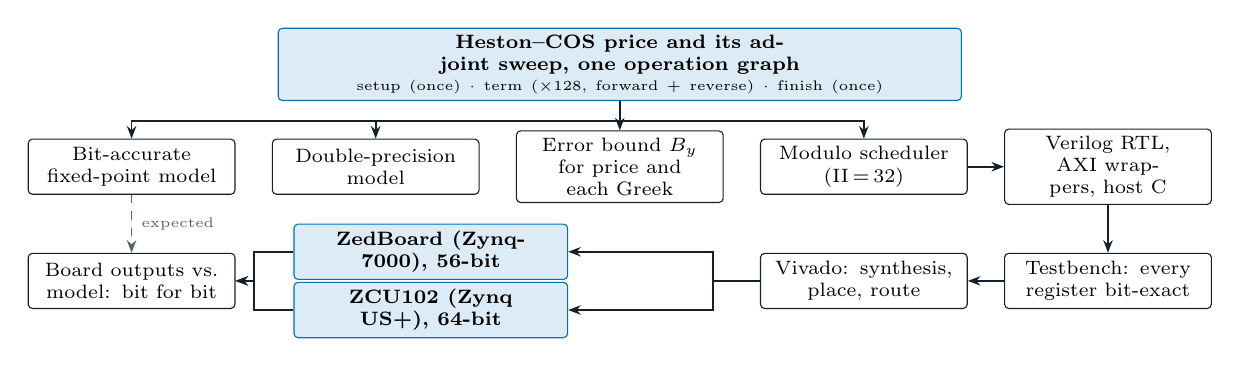
\begin{tikzpicture}[node distance=0.35cm]
  \node[key, text width=8.5cm] (src) at (0,0) {Heston--COS price and its adjoint sweep, one operation graph\\[-1pt]
    \normalfont\tiny setup (once) $\cdot$ term ($\times$128, forward + reverse) $\cdot$ finish (once)};
  \foreach \x/\n/\t in {-6.2/emu/{Bit-accurate\\fixed-point model}, -3.1/flt/{Double-precision\\model},
                        0/bnd/{Error bound $B_y$\\for price and each Greek}, 3.1/sch/{Modulo scheduler\\(II\,=\,32)}, 6.2/rtl/{Verilog RTL,\\AXI wrappers, host C}}
    \node[blk, text width=2.45cm] (\n) at (\x,-1.3) {\t};
  \foreach \n in {emu,flt,bnd,sch} \draw[arr] (src.south) -- ++(0,-0.25) -| (\n.north);
  \draw[arr] (sch) -- (rtl);
  \node[blk, text width=2.45cm] (tb) at (6.2,-2.75) {Testbench: every\\register bit-exact};
  \node[blk, text width=2.45cm] (viv) at (3.1,-2.75) {Vivado: synthesis,\\place, route};
  \node[key, text width=3.3cm, minimum height=0.5cm] (zed) at (-2.4,-2.38) {ZedBoard (Zynq-7000), 56-bit};
  \node[key, text width=3.3cm, minimum height=0.5cm] (zcu) at (-2.4,-3.12) {ZCU102 (Zynq US+), 64-bit};
  \node[blk, text width=2.45cm] (cmp) at (-6.2,-2.75) {Board outputs vs.\\model: bit for bit};
  \draw[arr] (rtl) -- (tb); \draw[arr] (tb) -- (viv);
  \draw[arr] (viv.west) -- ++(-0.6,0) |- (zed.east); \draw[arr] (viv.west) -- ++(-0.6,0) |- (zcu.east);
  \draw[arr] (zed.west) -- ++(-0.5,0) |- (cmp.east); \draw[arr] (zcu.west) -- ++(-0.5,0) |- (cmp.east);
  \draw[darr] (emu) -- node[lbl, right] {expected} (cmp);
\end{tikzpicture}
\caption{Design flow of the proposed accelerator. One operation graph yields the bit-accurate model, the error bound and the scheduled RTL, which is verified register by register, implemented in Vivado and validated bit for bit on two FPGA boards.}
\label{fig:flow}
\end{figure*}

\subsection{Co-Scheduled Adjoint Datapath}
Each COS term evaluates the payoff coefficient and the characteristic function (forward pass),
then propagates adjoints from the term's contribution back to the model inputs (reverse sweep),
normalises them by a power of two to keep small high-frequency adjoints at full precision, and
adds the results to nine accumulators (Fig.~\ref{fig:sched}, top). The computation contains no
data-dependent branches, so the lifetime of every forward value consumed by the reverse sweep is
known at design time. The modulo scheduler therefore allocates each such value a set of rotating
registers that carry it across the terms in flight: the tape is fixed in size (447 registers for
the 56-bit design), requires no memory, addressing or replay logic, and is read at exactly the
cycle each value is needed.

All arithmetic is mapped onto shared units: eight 56$\times$56-bit multipliers (nine DSP48E1 blocks
each), three CORDIC rotators and two CORDIC vectorers~\cite{volder}. Reciprocals and square roots use
Newton--Raphson iterations from table seeds and the exponential uses Tang's method~\cite{tang}, so
the datapath has no dividers. A COS term costs 250 multiplications, three rotations and two
vectorings, of which the price alone accounts for 126 multiplications. With 8 multipliers, 3
rotators and 2 vectorers, all three resource classes balance at an initiation interval (II) of
$\lceil 250/8\rceil = 3{\cdot}32/3 = 2{\cdot}32/2 = 32$ cycles, so a new term starts every 32 cycles
and about 16 terms are in flight (Fig.~\ref{fig:sched}, bottom). The CORDIC units set this pace, and
the reverse sweep's 124 additional multiplications per term occupy multiplier slots that the forward
pass leaves free. The 128-term loop completes in $127\cdot32+506+2=4{,}572$ cycles.

\begin{figure}[!t]
\centering
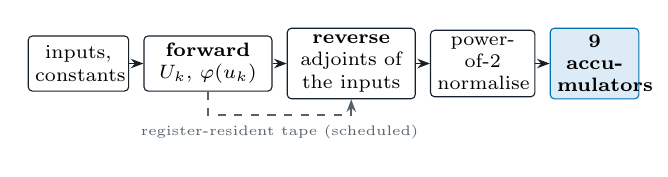
\begin{tikzpicture}[node distance=0.18cm]
  \node[blk, text width=1.1cm] (in) {inputs,\\constants};
  \node[blk, right=of in, text width=1.45cm] (fwd) {\textbf{forward}\\$U_k$, $\varphi(u_k)$};
  \node[blk, right=of fwd, text width=1.45cm] (rev) {\textbf{reverse}\\adjoints of\\the inputs};
  \node[blk, right=of rev, text width=1.15cm] (nrm) {power-of-2\\normalise};
  \node[key, right=of nrm, text width=0.95cm] (acc) {9 accu-\\mulators};
  \draw[arr] (in) -- (fwd); \draw[arr] (fwd) -- (rev); \draw[arr] (rev) -- (nrm); \draw[arr] (nrm) -- (acc);
  \draw[darr] (fwd.south) -- ++(0,-0.3) -| node[lbl, below, pos=0.25] {register-resident tape (scheduled)} (rev.south);
\end{tikzpicture}
\\[4pt]
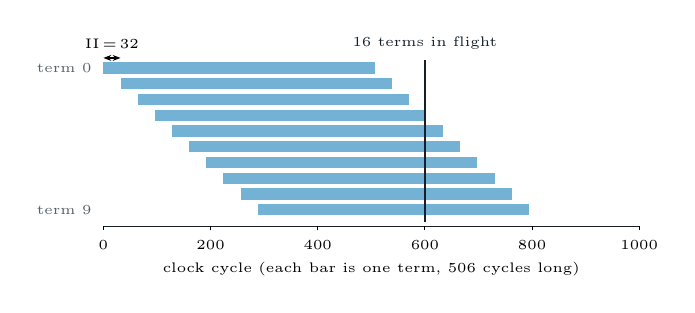
\begin{tikzpicture}[x=0.0068cm, y=0.2cm]
  \foreach \k in {0,...,9} {
    \pgfmathsetmacro{\s}{\k*32}
    \fill[acc!55] (\s, -\k) rectangle ++(506, 0.72);
  }
  \node[font=\tiny, text=muted, anchor=east] at (-4, 0.36) {term 0};
  \node[font=\tiny, text=muted, anchor=east] at (-4, -8.64) {term 9};
  \draw[ink, thick] (600,-9.4) -- (600,0.9) node[above, font=\tiny] {16 terms in flight};
  \draw[ink] (0,-9.7) -- (1000,-9.7);
  \foreach \c in {0,200,400,600,800,1000} { \draw (\c,-9.7) -- ++(0,-0.25) node[below, font=\tiny] {\c}; }
  \node[font=\tiny] at (500,-12.4) {clock cycle (each bar is one term, 506 cycles long)};
  \draw[{Stealth[length=1mm]}-{Stealth[length=1mm]}] (0,1.0) -- node[above, font=\tiny] {II\,=\,32} (32,1.0);
\end{tikzpicture}
\caption{Top: one COS term of the co-scheduled datapath; the reverse sweep reads forward values from scheduled rotating registers. Bottom: modulo schedule of the first 10 of 128 terms.}
\label{fig:sched}
\end{figure}

\subsection{Fixed-Point Arithmetic and Per-Greek Error Bound}
\label{sec:bound}
Values are two's-complement fixed point with $FL$ fraction bits: 56-bit words with $FL=28$ on the
Zynq-7000 and 64-bit words with $FL=32$ on the UltraScale+, rounded to nearest after every
operation. Data-dependent shifters are sized from ranges measured over the input domain, which
reduces logic by 35\%, and any input that would leave a measured range raises a
\texttt{range\_err} flag. With local errors $|\delta_i|\le\epsilon_i$ at operations $w_i$, the
first-order rounding error of every output $y$ obeys~\cite{linnainmaa}
\begin{equation}
|\hat y - y| \;\le\; \sum_i \left|\partial y/\partial w_i\right| \epsilon_i =: B_y .
\label{eq:bound}
\end{equation}
The sensitivities are computed by a reverse sweep over the graph, which itself includes the
hardware's adjoint operations, so $B_y$ bounds the rounding error of each Greek exactly as the
engine computes it. Newton--Raphson steps, table lookups and series terms appear as graph
operations with $\epsilon_i=2^{-(FL+1)}$; each CORDIC unit carries a measured local error
($2$\,ulp for rotation, and $2\max(1,1/|z|)$\,ulp for the vectoring angle). The bound is evaluated
at design time to select and certify the word length.

% =============================================================================
\section{FPGA Implementation}
Two configurations are implemented from the same generator. On the Xilinx Zynq-7000 (ZedBoard),
the 56-bit engine runs the 128-term loop in the programmable logic while the once-per-evaluation
setup and finish steps run as bit-exact generated C on the host. On the Zynq UltraScale+ (ZCU102),
a 64-bit engine with 32 multipliers computes the whole evaluation on chip in 1,593 cycles. Each
engine sits behind an AXI4-Lite register file and is driven over JTAG through a JTAG-to-AXI master,
so that board tests exercise the datapath directly. Fig.~\ref{fig:hw} shows the hardware setup,
and Table~\ref{tab:impl} summarises the post-route results.

\begin{figure}[!t]
\centering
% ---- replace this box with the photograph, e.g.
% \includegraphics[width=\columnwidth]{figures/hw_setup.jpg}
\fbox{\parbox[c][4.6cm][c]{0.94\columnwidth}{\centering\footnotesize\color{muted}
\textbf{[Hardware photograph to be inserted]}\\[4pt]
ZedBoard (Zynq-7000) and ZCU102 (Zynq UltraScale+)\\running the Greeks engine, with the JTAG/UART connections}}
\caption{Hardware setup: the ZedBoard and ZCU102 boards running the proposed Greeks accelerator.}
\label{fig:hw}
\end{figure}

\begin{table}[!t]
\centering
\caption{Post-Route Implementation Results}
\label{tab:impl}
\footnotesize
\setlength{\tabcolsep}{4pt}
\begin{tabular}{@{}lcc@{}}
\toprule
\textbf{Metric} & \textbf{Zynq-7000} & \textbf{Zynq US+}\\
& \textbf{(ZedBoard)} & \textbf{(ZCU102)}\\
\midrule
Device & xc7z020-1 & xczu9eg-2\\
Word length / multipliers & 56-bit / 8 & 64-bit / 32\\
LUT & 38,752 (72.8\%) & 77,515 (28.3\%)\\
FF & 32,134 (30.2\%) & 63,547 (11.6\%)\\
DSP & 72 (32.7\%) & 510 (20.2\%)\\
BRAM tiles & 4.5 (3.2\%) & 7.5 (0.8\%)\\
Clock (MHz); WNS (ns) & 70; +0.458 & 100; +1.601\\
Cycles per evaluation & 4,572 (loop) & 1,593 (whole)\\
Latency, price + 9 Greeks & 65.3\,$\mu$s & 15.9\,$\mu$s\\
Power, engine$^{a}$ & 0.676\,W & 2.485\,W\\
Energy per evaluation & 44\,$\mu$J & 40\,$\mu$J\\
\bottomrule
\end{tabular}
\par\vspace{2pt}\parbox{\columnwidth}{\scriptsize $^{a}$On-chip power of the routed engine from gate-level switching activity on bit-exact evaluations, including device static power. Resources include the JTAG-to-AXI test system.}
\end{table}

% =============================================================================
\section{Results}
\subsection{Cost of the Greeks}
Fig.~\ref{fig:cycles} compares cycles per evaluation on identical fabric. A price-only engine
reaches II\,$=$\,32 with four multipliers; the adjoint engine delivers the price and nine Greeks at
the same throughput in 4,733 instead of 4,613 cycles, a 3\% increase, while bump-and-reprice
requires 86,860 cycles (18.4$\times$). On the 64-bit configuration the corresponding figures are
1,593, 1,540 and 19,562 cycles. Table~\ref{tab:equal} reports the three engines of equal throughput
implemented in Vivado on the Zynq-7000. The nine Greeks add 1.68$\times$ the LUTs and 2$\times$ the
DSP blocks of the price-only engine at 1.03$\times$ its cycles. Obtaining the same Greeks from the
price-only engine by bump-and-reprice takes 19 runs per option, so the adjoint engine delivers about
11$\times$ more priced-and-differentiated options per unit area and time.

\begin{figure}[!t]
\centering
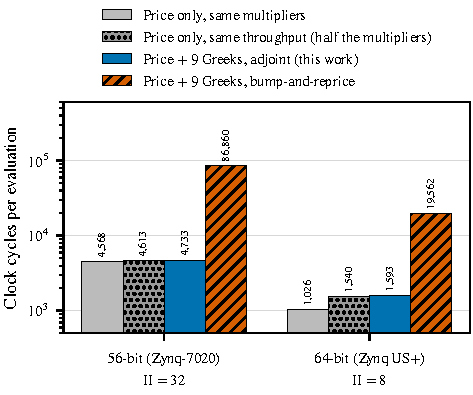
\includegraphics[width=\columnwidth]{fig_cycles.pdf}
\caption{Cycles per evaluation: price only (same multipliers, and same throughput with half the multipliers), the proposed adjoint engine, and bump-and-reprice on the same fabric.}
\label{fig:cycles}
\end{figure}

\begin{table}[!t]
\centering
\caption{Engines of Equal Throughput (II = 32) on Zynq-7000 at 70\,MHz}
\label{tab:equal}
\footnotesize
\setlength{\tabcolsep}{2.4pt}
\begin{tabular}{@{}lrrrrrr@{}}
\toprule
\textbf{Engine} & \textbf{Mult.} & \textbf{LUT} & \textbf{FF} & \textbf{DSP} & \textbf{Cycles} & \textbf{Greek err.}\\
\midrule
Price only & 4 & 21,251 & 15,303 & 36 & 4,457 & ---\\
\textbf{Adjoint (proposed)} & \textbf{8} & \textbf{35,782} & \textbf{27,204} & \textbf{72} & 4,572 & $\mathbf{1.2\times10^{-5}}$\\
Forward, factored & 10 & 38,199 & 30,514 & 90 & 4,449 & $7.4\times10^{-5}$\\
\bottomrule
\end{tabular}
\par\vspace{2pt}\parbox{\columnwidth}{\scriptsize Out-of-context implementations; all three verified bit-exact against their models. Greek err.: worst relative error of any Greek over 21 test cases.}
\end{table}

\subsection{Adjoint Against Forward Mode}
Three forward-mode datapaths were generated from the same primitives and scheduler: dense (as a
vector forward-mode tool builds it), sparse (structural zeros removed) and factored (exponent
derivatives shared per term, as a hand derivation of analytic Greeks does). Per COS term they
need 802, 396 and 313 multiplications against the adjoint's 250. At equal throughput
(Table~\ref{tab:equal}) the factored forward engine requires 6.8\% more LUTs, 12.2\% more
flip-flops and 25\% more DSP blocks, and, carrying its tangents without per-term rescaling, it is
6$\times$ less accurate at the same word length.

\subsection{Accuracy and Error Bound}
On a 21-case grid the 56-bit engine computes the price to within $6.1\times10^{-7}$ and every
Greek to within $1.2\times10^{-5}$ relative error of the same algorithm in double precision;
the 64-bit engine is one to two orders of magnitude more accurate. No output exceeds 0.103 of
its bound on the grid, 0.378 over a 10,500-input sweep including seven
hard regimes (Feller-violating, extreme correlation, deep strikes, short and long maturities, high
vol-of-vol, low variance), or 0.356 on a further held-out sweep of 10,500 inputs. A 50-digit
re-evaluation confirms the first-order assumption: the hardware error stays within 0.24 of the
bound. Against bump-and-reprice on the same pricer and word length (Fig.~\ref{fig:bump}), the
adjoint Greeks are 32--560$\times$ more accurate (median 145$\times$) than the best bump size chosen
separately for each Greek, without any tuning. The rounding bound complements the COS
discretisation error, which is controlled by the number of terms $N$.


\begin{figure*}[!t]
\centering
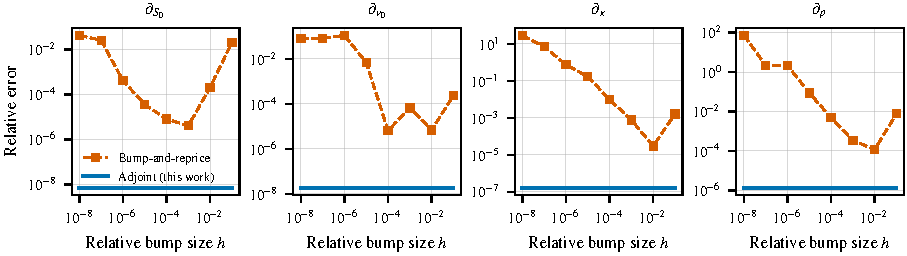
\includegraphics[width=\textwidth]{fig_bump.pdf}
\caption{Relative error of bump-and-reprice against bump size, and of the proposed adjoint engine, for four representative Greeks (56-bit, base case).}
\label{fig:bump}
\end{figure*}

\subsection{Silicon Validation}
The engines were run back to back without reset on both boards (Table~\ref{tab:silicon}),
including 50 Heston parameter sets calibrated to NIFTY index options. All 1,469 outputs matched
the bit-accurate model exactly, so every accuracy result and the error bound carry over to
silicon; the largest error-to-bound ratio measured on hardware is 0.255.

\begin{table}[!t]
\centering
\caption{Silicon Validation (Outputs Compared Bit for Bit with the Model)}
\label{tab:silicon}
\footnotesize
\setlength{\tabcolsep}{3pt}
\begin{tabular}{@{}llrrc@{}}
\toprule
\textbf{Board} & \textbf{Input set} & \textbf{Cases} & \textbf{Bit-exact} & \textbf{Err./bound}\\
\midrule
ZedBoard & reference + random & 51 & 459 / 459 & 0.199\\
ZCU102 & reference + random & 51 & 510 / 510 & 0.243\\
ZCU102 & NIFTY calibrations & 50 & 500 / 500 & 0.255\\
\midrule
\multicolumn{3}{@{}l}{\textbf{Total}} & \textbf{1,469 / 1,469} & $\le$\,0.255\\
\bottomrule
\end{tabular}
\end{table}

\subsection{Comparison with Software and Prior FPGA Work}
Table~\ref{tab:cpu} places the engine against the same algorithm on a laptop CPU (Intel
i5-1155G7, double precision). The UltraScale+ engine computes the price and nine Greeks
4.9$\times$ faster than forward-mode AD, 6.5$\times$ faster than taped AAD (CoDiPack~\cite{codipack})
and 15$\times$ faster than bump-and-reprice on one core, and matches hand-optimised analytic Greeks
within 1.2$\times$ in latency at the same energy per evaluation (40 against 40.9\,$\mu$J), with a
fixed, input-independent cycle count. Table~\ref{tab:compare} compares the design with FPGA engines
from the literature: it is the only one to compute Greeks by an adjoint, the only one using a
Fourier method, and the only one that attaches an accuracy guarantee to each Greek.

\begin{table}[!t]
\centering
\caption{Price and Nine Greeks: FPGA Engine Versus CPU Implementations}
\label{tab:cpu}
\footnotesize
\setlength{\tabcolsep}{2.2pt}
\begin{tabular}{@{}lrrr@{}}
\toprule
\textbf{Implementation} & \textbf{Latency} & \textbf{Cost vs.} & \textbf{Energy}\\
& \textbf{($\mu$s)} & \textbf{price} & \textbf{($\mu$J)}\\
\midrule
CPU, bump-and-reprice & 238.1 & 17.4$\times$ & ---\\
CPU, taped AAD (CoDiPack) & 103.8 & 7.6$\times$ & ---\\
CPU, forward-mode AD & 78.0 & 5.7$\times$ & ---\\
CPU, analytic Greeks (vectorised) & 13.6 & --- & 40.9$^{a}$\\
\midrule
\textbf{FPGA, Zynq-7000 (proposed)} & \textbf{65.3} & \textbf{1.04$\times$} & \textbf{44}\\
\textbf{FPGA, Zynq US+ (proposed)} & \textbf{15.9} & \textbf{1.55$\times$} & \textbf{40}\\
\bottomrule
\end{tabular}
\par\vspace{2pt}\parbox{\columnwidth}{\scriptsize CPU: Intel i5-1155G7, g++ -O3, one core; latency is the best of five runs. $^{a}$Measured package power at full four-core throughput. Cost: time relative to the price alone on the same platform. FPGA latency from the cycle count at the operating clock.}
\end{table}

\begin{table*}[!t]
\centering
\caption{Comparison With FPGA Option-Pricing and Greeks Engines}
\label{tab:compare}
\footnotesize
\setlength{\tabcolsep}{4pt}
\begin{tabular}{@{}L{2.6cm}C{3.4cm}C{3.5cm}C{2.9cm}C{3.2cm}@{}}
\toprule
\textbf{Metric} & \textbf{Proposed} & \textbf{Klaisoongnoen et al.~\cite{klai,klaih2rc}} & \textbf{AMD Vitis Quant.~\cite{vitisquant}} & \textbf{de Schryver et al.~\cite{deschryver13}}\\
\midrule
Model & Heston & Heston (STAC-A2) & Heston & Heston\\
Pricing method & COS (Fourier) & Monte Carlo + Longstaff--Schwartz & Monte Carlo & Multi-level Monte Carlo\\
Greeks computed by & \textbf{Adjoint, one pass} & Re-simulation (finite differences) & Central differences & --- (price only)\\
Greeks cost vs.\ price & \textbf{1.03$\times$ (equal throughput)} & N/R & 19 pricings & ---\\
Arithmetic & 56/64-bit fixed point & Double, single, half, fixed (explored) & Floating point & N/R\\
Accuracy guarantee & \textbf{Per-Greek rounding bound} & None & None & None\\
Platform & Zynq-7000, Zynq US+ & Alveo U280, Stratix-10 & Alveo & Virtex-6\\
Silicon-validated & Yes, bit-exact & Yes & Library & Yes\\
Reported result & 15.9\,$\mu$s, 40\,$\mu$J per price + 9 Greeks & 8--185$\times$ efficiency vs.\ 2$\times$ Xeon 8260M & N/R & $\approx$100 M steps/s at 3.58\,W\\
\bottomrule
\end{tabular}
\par\vspace{2pt}\parbox{\textwidth}{\scriptsize N/R: not reported. Reported results are each work's own headline metric and are not directly comparable across pricing methods.}
\end{table*}

% =============================================================================
\section{Conclusion}
This work presented an FPGA accelerator that computes Heston option prices and all nine
first-order Greeks by adjoint differentiation. By co-scheduling the reverse sweep with the
forward COS pass in a single fixed-point datapath, with its stored values in a register-resident
tape, the engine delivers the Greeks for 1.03$\times$ the cycles of a price-only engine of equal
throughput, needs 18.4$\times$ fewer cycles than bump-and-reprice and 25\% fewer DSP blocks than
forward mode, and is 32--560$\times$ more accurate than bumping. A per-Greek rounding-error bound,
never exceeded over 21,000 inputs, accompanies every output, and bit-exact operation was confirmed
on Zynq-7000 and Zynq UltraScale+ silicon with real market calibrations. Automatic derivation of
the reverse sweep in the generator and multi-lane engines for lower latency are directions for
future work.

% =============================================================================
\begin{thebibliography}{99}
\bibitem{heston} S.~L. Heston, ``A closed-form solution for options with stochastic volatility with applications to bond and currency options,'' \emph{Rev. Financial Stud.}, vol.~6, no.~2, pp.~327--343, 1993.
\bibitem{fang} F.~Fang and C.~W. Oosterlee, ``A novel pricing method for European options based on Fourier-cosine series expansions,'' \emph{SIAM J. Sci. Comput.}, vol.~31, no.~2, pp.~826--848, 2008.
\bibitem{deschryver} C.~de~Schryver \emph{et~al.}, ``An energy efficient FPGA accelerator for Monte Carlo option pricing with the Heston model,'' in \emph{Proc. Int. Conf. Reconfigurable Computing and FPGAs (ReConFig)}, 2011.
\bibitem{deschryver13} C.~de~Schryver, P.~Torruella, and N.~Wehn, ``A multi-level Monte Carlo FPGA accelerator for option pricing in the Heston model,'' in \emph{Proc. Design, Automation \& Test in Europe (DATE)}, 2013, pp.~248--253.
\bibitem{jin} Q.~Jin, D.~B. Thomas, W.~Luk, and B.~Cope, ``Exploring reconfigurable architectures for tree-based option pricing models,'' \emph{ACM Trans. Reconfigurable Technol. Syst.}, vol.~2, no.~4, art.~21, 2009.
\bibitem{tse} A.~H.~T. Tse, D.~Thomas, and W.~Luk, ``Design exploration of quadrature methods in option pricing,'' \emph{IEEE Trans. Very Large Scale Integr. (VLSI) Syst.}, vol.~20, no.~5, pp.~818--826, 2012.
\bibitem{klai} M.~Klaisoongnoen, N.~Brown, and O.~Thomson~Brown, ``Low-power option Greeks: Efficiency-driven market risk analysis using FPGAs,'' in \emph{Proc. Int. Symp. Highly-Efficient Accelerators and Reconfigurable Technologies (HEART)}, 2022, pp.~95--101.
\bibitem{klaih2rc} M.~Klaisoongnoen, N.~Brown, and O.~Thomson~Brown, ``Fast and energy-efficient derivatives risk analysis: Streaming option Greeks on Xilinx and Intel FPGAs,'' in \emph{Proc. Int. Workshop Heterogeneous High-Performance Reconfigurable Computing (H2RC), SC22}, 2022.
\bibitem{klai24} M.~Klaisoongnoen, N.~Brown, T.~Dykes, J.~R. Jones, and U.-U. Haus, ``Evaluating Versal AI Engines for option price discovery in market risk analysis,'' in \emph{Proc. ACM/SIGDA Int. Symp. Field-Programmable Gate Arrays (FPGA)}, 2024.
\bibitem{vitisquant} AMD, ``Vitis Libraries: Quantitative Finance Library,'' [Online]. Available: \url{https://github.com/Xilinx/Vitis_Libraries}
\bibitem{giles} M.~Giles and P.~Glasserman, ``Smoking adjoints: Fast Monte Carlo Greeks,'' \emph{Risk}, vol.~19, pp.~88--92, Jan. 2006.
\bibitem{capriotti} L.~Capriotti, ``Fast Greeks by algorithmic differentiation,'' \emph{J. Comput. Finance}, vol.~14, no.~3, pp.~3--35, 2011.
\bibitem{capgiles24} L.~Capriotti and M.~Giles, ``15 years of adjoint algorithmic differentiation (AAD) in finance,'' \emph{Quant. Finance}, vol.~24, no.~9, pp.~1353--1379, 2024.
\bibitem{albrecher} H.~Albrecher, P.~Mayer, W.~Schoutens, and J.~Tistaert, ``The little Heston trap,'' \emph{Wilmott Mag.}, pp.~83--92, Jan. 2007.
\bibitem{griewank} A.~Griewank and A.~Walther, \emph{Evaluating Derivatives: Principles and Techniques of Algorithmic Differentiation}, 2nd~ed. Philadelphia, PA, USA: SIAM, 2008.
\bibitem{tapenade} L.~Hasco\"et and V.~Pascual, ``The Tapenade automatic differentiation tool: Principles, model, and specification,'' \emph{ACM Trans. Math. Softw.}, vol.~39, no.~3, 2013.
\bibitem{cui} Y.~Cui, S.~del~Ba\~no~Rollin, and G.~Germano, ``Full and fast calibration of the Heston stochastic volatility model,'' \emph{Eur. J. Oper. Res.}, vol.~263, no.~2, pp.~625--638, 2017.
\bibitem{zhang09} B.~Zhang and C.~W. Oosterlee, ``Option pricing with COS method on graphics processing units,'' in \emph{Proc. IEEE Int. Symp. Parallel \& Distributed Processing (IPDPS)}, 2009, pp.~1--8.
\bibitem{zhang14} B.~Zhang and C.~W. Oosterlee, ``Acceleration of option pricing technique on graphics processing units,'' \emph{Concurrency Computat.: Pract. Exper.}, vol.~26, no.~9, pp.~1626--1639, 2014.
\bibitem{gaffar} A.~A. Gaffar, O.~Mencer, W.~Luk, P.~Y.~K. Cheung, and N.~Shirazi, ``Floating-point bitwidth analysis via automatic differentiation,'' in \emph{Proc. IEEE Int. Conf. Field-Programmable Technology (FPT)}, 2002, pp.~158--165.
\bibitem{lee06} D.-U. Lee, A.~A. Gaffar, R.~C.~C. Cheung, O.~Mencer, W.~Luk, and G.~A. Constantinides, ``Accuracy-guaranteed bit-width optimization,'' \emph{IEEE Trans. Comput.-Aided Design Integr. Circuits Syst.}, vol.~25, no.~10, pp.~1990--2000, 2006.
\bibitem{rau} B.~R. Rau, ``Iterative modulo scheduling: An algorithm for software pipelining loops,'' in \emph{Proc. 27th Annu. Int. Symp. Microarchitecture (MICRO)}, 1994, pp.~63--74.
\bibitem{volder} J.~E. Volder, ``The CORDIC trigonometric computing technique,'' \emph{IRE Trans. Electron. Comput.}, vol.~EC-8, no.~3, pp.~330--334, 1959.
\bibitem{tang} P.~T.~P. Tang, ``Table-driven implementation of the exponential function in IEEE floating-point arithmetic,'' \emph{ACM Trans. Math. Softw.}, vol.~15, no.~2, pp.~144--157, 1989.
\bibitem{linnainmaa} S.~Linnainmaa, ``Taylor expansion of the accumulated rounding error,'' \emph{BIT Numer. Math.}, vol.~16, no.~2, pp.~146--160, 1976.
\bibitem{codipack} M.~Sagebaum, T.~Albring, and N.~R. Gauger, ``High-performance derivative computations using CoDiPack,'' \emph{ACM Trans. Math. Softw.}, vol.~45, no.~4, 2019.
\end{thebibliography}

\end{document}
